\documentclass[12pt]{article}

\setlength{\oddsidemargin}{-0.25 in}
\setlength{\evensidemargin}{-0.25 in}
\setlength{\topmargin}{-0.9 in}
\setlength{\textwidth}{7.0 in}
\setlength{\textheight}{9.0 in}
\setlength{\headsep}{0.75 in}
\setlength{\parindent}{0.0 in}
\setlength{\parskip}{0.0 in}

\usepackage{graphicx}
\usepackage{multirow}
\usepackage[table]{xcolor}

\begin{document}
\begin{center}
Classifying Malicious Software \\
Ryan Kerr, Tony Li, George Zhang \\ 
CS181 Practical 2 Writeup \\
https://github.com/gzhang01/cs181practicals/tree/master/practical2 \\
\end{center}

\bigskip
\bigskip

\textbf{Abstract} \\
Our task was to classify executable files into one of 14 known malware classes or determine that the executable was not malware. To accomplish this, we investigated different classifiers as well as extracted various sets of features. Our goal was to improve our classification accuracy by both selecting the best classifier and using the most informative features. Ultimately, we settled on a random forest classifier with 40 estimators and used a set of 22 features extracted from the XML files. This model resulted in an accuracy of 80.6\% when predicting on the test data, according to Kaggle. \\

\bigskip

\textbf{Technical Approach} \\
After receiving our task, we decided that we would tackle this problem using a two-pronged approach: we would attempt to extract features that provide useful information for classification, and we would experiment with different classifiers to identify which would do the best with a given set of features. Thus we began by collecting some sample features that we could test different classifiers with and found a sample classifier that we could test different sets of features on. We wrote a script modeled after the sample code that extracted a total of 5 system calls (dump\_line, download\_file, open\_file, connect\_socket, impersonate\_user). We also implemented a test suite that used cross validation with a Gaussian Naive Bayes classifier (from sklearn) as a sample. With this starting point, we attempted to find additional features and better classifiers.  \\

We investigated various classifiers from sklearn, including the random forest classifier, adaboost classifier, bagging classifer, and extra trees classifier. We also tested our Gaussian generative model from the previous homework. For the ones from sklearn (except Naive Bayes), we also ran trials on differing numbers of estimators to see how many estimators produced the best results given a set of features. The results of these tests are listed in detail under results. Ultimately, we found that the random forest classifier with 40 estimators performed the best overall, and so we produced our predictions with that model. \\

We also attempted to find some more effective features. Our initial five did rather poorly with our initial tests. When we extracted another 8, mostly from looking through the XML files and seeing what system calls were made and using what we thought might be helpful, we produced significantly better results. Unfortunately, this method only got us so far once we started using the random forest generator to test our features. Eventually we were unable to produce more significant improvements. We did, however, change the way we extracted the features from the XML files. The sample code produced an element tree and pulled system calls off of it. We ended up converting the tree to a string and used regular expressions to match certain substrings we were interested in. This allowed us to extract features that were not limited to system calls and their arguments, but also included substrings of arguments. 

\bigskip

\textbf{Results} \\
After expanding our feature set, we ran several tests in an attempt to identify a good classifier to proceed with. Running cross-validation with 20 blocks, we got the following data:

\begin{table}[h!]
\centering
\begin{tabular} {c | c | c}
Classifier & Mean (\%) & Std Dev (\%) \\ \hline
Gaussian Generative Model & 37.66 & 10.17 \\
Gaussian Naive Bayes & 26.46 & 4.41 \\
Random Forest Classifier & \cellcolor{green}88.54 & \cellcolor{green}2.16 \\
AdaBoost Classifier & 68.93 & 3.09 \\
Bagging Classifier & 87.89& 2.38 \\
Extra Trees Classifier & \cellcolor{green}88.80 & 2.56 \\
\end{tabular}
\caption{Cross-validation Results with Different Classifiers (n = 20)}
\label{table:1}
\end{table}

A few notes before we take a closer look at the data. First, the Gaussian generative model came from the previous homework. All the other models came from sklearn. Also, the means we found from this cross-validation procedure appear to be inflated. When we made predictions for the test data using the random forest generator with the same set of features that produced these results, Kaggle gave us an accuracy of 80\%, which is far less than the 88.54\% we saw with our test suite. We currently do not have a good explanation for this. As a result, for most of our analysis, we focused less on the actual value produced but on the change in value that resulted from various actions. \\

We noticed that the random forest classifier and the extra trees classifier did pretty well compared with the rest of the models. However, the random forest classifier had a lower standard deviation than the extra trees classifier. Because of this, we decided to do the bulk of our testing with the random forest classifier. \\

We also took a look at how changing the number of classifiers would affect the model. For each of the last four models, we ran the test suite using various numbers of classifiers (N = 2, 5, 10, 20, 30, 40, 50, 70, 90). We graphed the results: \\\\

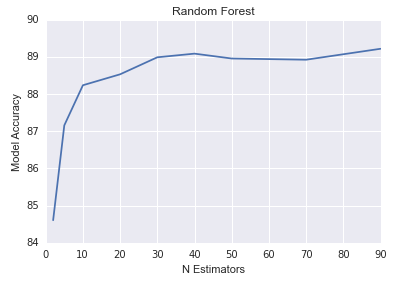
\includegraphics[width=0.5\textwidth]{img/RandomForest.png}
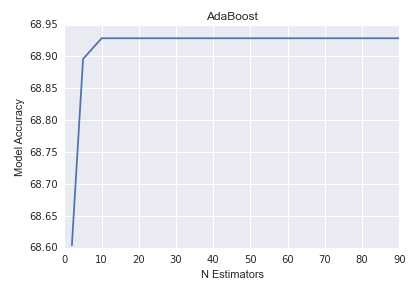
\includegraphics[width=0.5\textwidth]{img/AdaBoost.png} \\
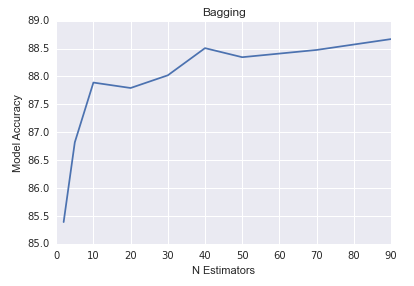
\includegraphics[width=0.5\textwidth]{img/Bagging.png}
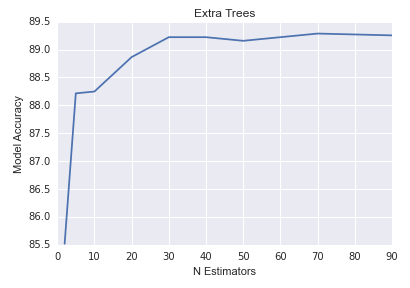
\includegraphics[width=0.5\textwidth]{img/ExtraTrees.png} \\

Again, these graphs show that random forests and extra trees performed better than the other two. In addition, we found that random trees performed well in our cross-validation when the number of estimators was 40. \\

In addition to finding better classifiers, we also attempted to find better features. Our initial 5 did relatively poorly (accuracy $\approx$ 14\% with Gaussian generative model). With our expanded list of features, which we used for testing the classifiers, we managed to improve the Gaussian generative model to an accuracy of 37.66\%. After running the tests on classifiers, we transitioned to using the random forest classifier to test our features, so our baseline became 88.54\%. We found that further feature engineering did not produce particularly significant improvements beyond that. With our final feature set, the random forest classifier running with 40 estimators produced a mean accuracy of 89.29\%. 

With our feature set (num = 22) and our model, we submitted predictions for classes based on the test data. According to Kaggle, our accuracy was 80.6\%.

\bigskip

\textbf{Discussion} \\
Since the only data we had to start was the XML files from the training and testing data, our first task was to extract some features so we had something to work with in our classification problem. We initially extracted 5 features just so we had something to work with, and from there, we built a test suite that we could use for evaluating our model without having to upload to Kaggle. Our initial attempts with Naive Bayes and Gaussian generative model produced fairly poor results, which prompted us to find better classifiers as well as better features. \\

We had the most success with ensemble methods. Running a variety of classifiers on an expanded set of features revealed that random forest classifiers worked best. We then experimented with the number of estimators, and graphed the results so we could easily visualize the data. From this, we concluded that the best model to use was the random forest classifier with 40 estimators.  \\

We also approached the problem from a feature engineering angle. We believed that our poor initial performance was the result of poor features as much as poor classifier. Thus we attempted to find better features that provided more information for our classifier. Initially, this process worked well. Adding addition features resulted in much improvement in our performance. As a result, we decided to simply add more, but soon, the benefit started plateauing and, especially after we transitioned to using random forests, we decided that we needed a smarter way to find our features. We ended up extracting substrings, as described in the technical approach, which provided us with a slightly different subset of features than what was available with just system calls. In addition, we ended up pruning our features by examining the relative performance benefit with and without the given feature and narrowed our set of features down to 22 which we felt confident contributed positively to our prediction. This set of features eventually went into our final prediction. \\

\bigskip

\textbf{Conclusion} \\
We were tasked with classifying executable files into classes of malware or determining that it was not malware. Our approach included feature engineering and evaluating different classifiers to find the combination that would provide us with the best results. We were ultimately able to produce a model that had a 80.6\% accuracy rate using a random forest classifier with 40 estimators and a set of 22 features. With more time, we would have liked to look into ways to use neural networks, which hopefully would have produced features that were more informative. 


\end{document}








